% ===================================================================
% Arquivo: capitulos/parte-III-pilares/cap-09-modernas.tex
% ===================================================================

\chapter{Funções de Ativação Modernas e Outras Funções de Ativação}
\label{cap:ativacao-modernas-outras}

\section{Funções Modernas: O Estado-da-Arte das Funções de Ativação}

\subsection{Gaussian Error Linear Unit (GELU)} \index{Funções de Ativação!Gaussian Error Linear Unit (GELU)}

Agora chegamos na última função que iremos ver neste texto, ela é a Gaussian Error Linear Unit, ou GELU. Ela é uma das mais diferentes quando nós passamos a analisar como é sua fórmula, a qual veremos mais em frente. A GELU foi introduzida no artigo \textit{Gaussian Error Linear Units (GELUs)} dos autores \textcite{GELUArticle}, nele, os pesquisadores apresentam uma nova função de ativação de alta performance para ser utilizada na construção de redes neurais.

No texto, os autores, avaliam a GELU e outras variantes como a Exponential Linear Unit e a ReLU tradicional no dataset MNIST, o qual apresenta 10 classes de imagens em escala de cinza sendo 60.000 imagens de treino e 10.000 de teste, os resultados de como a perda e robustez a ruído dessas funções se comporta o longo do experimento podem ser vistos nas figuras \ref{fig:log-loss-gelu} e \ref{fig:accuracy-gelu} respectivamente \parencite{GELUArticle}. Além disso, \textcite{GELUArticle}, avaliaram essas funções em outros conjuntos como o MNIST autoencoding, Tweet part-of-speech tagging, TIMIT frame recognition além dos datasets de imagens CIFAR-10/100. 

Analisando a figura \ref{fig:log-loss-gelu}, podemos compreender como essas diferentes funções contribuem para a diminuição da perda no modelo criado para a classificação do dataset MNIST. Nos vemos que a GELU é a função que apresenta a menor perda, mas não somente isso, ela é a que contribui para que ela diminua mais rapidamente. Nos casos em que foi utilizado o dropout nas camadas os resultados são ainda mais mais significativos, com a ReLU apresentando a maior perda dentre as três funções, a ELU em segundo, e GELU com uma diferença considerável em relação as suas concorrentes. Isso pode nos indicar que em redes neurais cujo técnicas como o dropout de neurônios nas camadas não seja uma prática viável, pode ser interessante utilizar como estratégia a GELU como função de ativação, pois mesmo sem o dropout, ela consegue manter um bom valor para a perda do modelo que está sendo desenvolvido.

Já na figura \ref{fig:accuracy-gelu}, podemos ver como a acurácia dos modelos se comporta quando é adicionado é adicionado ruído as dados de teste. Para isso, nós notamos que os todos os modelos possuem a mesma tendência de decrescer a sua acurácia ao longo do aumento do ruído, vemos que o modelo que é mais afetado com essa transformação é o que faz uso da exponential linear unit, enquanto os que fazem uso da ReLU e da GELU, mesmo encontrando grandes dificuldades para identificar coretamente as imagens, conseguem manter uma acurácia de quase 0.1 a mais que a ELU. Ainda na figura \ref{fig:accuracy-gelu}, também vemos como a perda no conjunto de testes de comporta ao aumentar o ruído, aqui vemos uma situação diferente, vemos que o modelo que menos se adequou ao que estava analisando foi o que fazia uso da ReLU, pois, encontrou difuculdades em tentar minizar o cálculo da perda, por outro lado temos a GELU, que mesmo aumentando o ruído, conseguiu manter uma diferença considerável quando comparada a essas outras duas funções.

Além disso, como dito anteriormente, os autores também fazem testes comparando a GELU com outras funções de ativação utilizando também o dataset CIFAR-10, o qual vem sendo discutido em seções anteriores deste texto, assim, temos a figura \ref{fig:gelu-cifar-10}, que nos mostra esse comparativo com a taxa de erro \parencite{GELUArticle}. Com base nessa análise, nós podemos concluir que a GELU é a melhor alternativa dentre essas três funções para a rede que foi criada, apresentando a menor taxa de erro, tanto no conjunto de dados de treino quanto no conjunto de dados de teste. Uma observação interessante a ser feita com base neste gráfico é de que esses modelos foram treinados por 200 épocas no total, e como a GELU é uma função bem mais complexa que a ReLU, o tempo de treino do modelo que fez uso dessa função foi provavelmente bem maior, algo que pode ser levado em consideração caso seja necessário criar uma rede que seja treinada mais rapidamente mas que ainda sim tenha uma taxa de erro baixa.

Conhecendo um pouco como a GELU atua em uma rede neural, podemos agora conhecer ela por meio da sua fórmula, a qual é dada pela expressão \ref{eq:gelu}, a qual é um tanto diferente das outras expressões que vimos até agora. Note que nós não temos dessa vez uma expressão condicional como na ReLU e suas outras variantes, temos uma expressão única, que pode ser reescrita utilizando outras expressões diferentes. Mais a esquerda, temos o termo $\Phi(z_i)$ que representa o standard Gaussian cumalative distribution function, já na expressão mais a direita, temos o uso da função erro, uma função bem comum de ser utilizada quando estamos trabalhando com conceitos probabilísticos.

\begin{equacaodestaque}{Gaussian Error Linear Unit}
    \mathcal{A}_{\text{GELU}}(z_i) = z_i P(X \leqslant z_i) = z_i \Phi (z_i) = z_i \frac{1}{2} \left[ 1 + \text{erf} (z_i/ \sqrt{2}) \right]
    \label{eq:gelu}
\end{equacaodestaque}

Por apresentar cálculos mais complexos em sua composição, como o uso da função erro para encontrar o satrd gaussian cumative distribution function os autores também apresentam aproximações para a GELU, elas são dadas pelas equações \ref{eq:EquacaoGELUAprox} e \ref{eq:EquacaoGELUAprox2} \parencite{GELUArticle}. Essas aproximações facilitam não somente os cálculos mas também na hora de implementar essa função em Python, garantindo algoritmos mais curtos e fáceis de serem implementados.

Na expressão \ref{eq:gelu-aproximacoes} vemos que ela pode ser aproximada utilizando a função tangente como um dos componentes usados, já na expressão \ref{eq:gelu-aproximacoes-sigmoide}, os autores utilizam como base a Sigmoid Linear Unit (SiLU), a qual é dada pela fórmula $SiLU = x\sigma(x)$ para criar uma expressão que seja capaz de aproximar como a GELU se comporta mas trazer uma maior velocidade de processamento por apresentar cálculos mais simples em sua composição.
    
\begin{equacaodestaque}{Gaussian Error Linear Unit Aproximações}
    \mathcal{A}_{\text{GELU}(x)} \approx 0.5x \left(1 + \tanh\left[\sqrt{\frac{2}{\pi}} \left(x + 0.044715x^3\right)\right]\right) \\
    \label{eq:gelu-aproximacoes}
\end{equacaodestaque}

\begin{equacaodestaque}{Gaussian Error Linear Unit Aproximação com Sigmoide}
    \mathcal{A}_{\text{GELU}}(x) \approx x \sigma(1.702x)
    \label{eq:gelu-aproximacoes-sigmoide}
\end{equacaodestaque}

Se sabemos a sua fórmula, podemos também plotar o seu gráfico, para isso temos a figura \ref{fig:gelu}, esse gráfico é uma aproximação, tendo como base a expressão \ref{eq:gelu-aproximacoes}. Note que ela é uma função assimétrica, que possui o comportamento quase que de uma função identidade para os casos em que a sua entrada é maior que zero, além disso, podemos ver que ela retorna valores não nulos quando a entrada é negativa, mas apenas até um certo ponto, depois ela assume o comportamento de um função constante. O fato dela retornar valores quando alguns valores da entrada são negativos pode acabar contribuindo para que essa função diminua o problema do neurônios agonizantes, além disso, por ser uma variante da ReLU, ela também é capaz de resolver o problema do gradiente em fuga.

\begin{figure}[htbp]
    \centering
    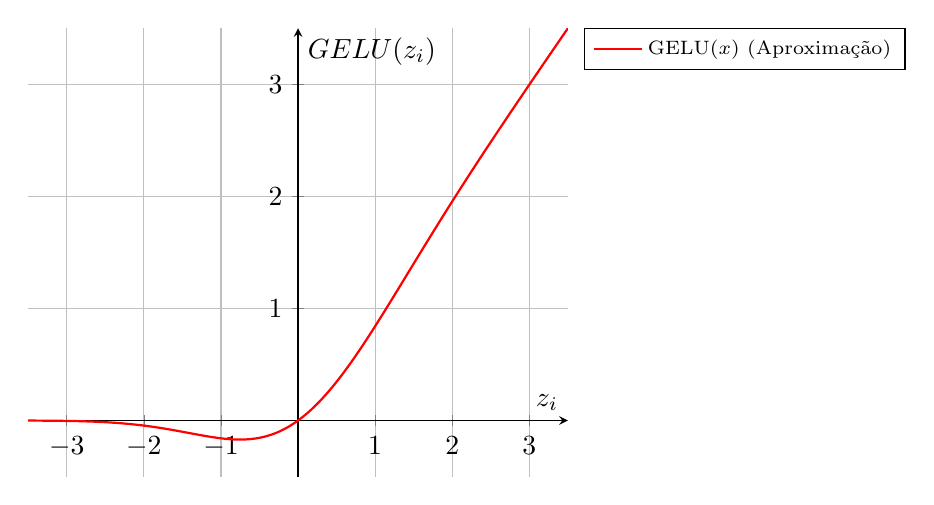
\begin{tikzpicture}
        \begin{axis}[
            xlabel={$z_i$},
            ylabel={$\text{GELU}(z_i)$},
            xmin=-3.5, xmax=3.5,
            ymin=-0.5, ymax=3.5,
            axis lines=middle,
            grid=major,
            legend pos=outer north east,
            legend style={font=\scriptsize}
        ]
        % Plota a APROXIMAÇÃO da função GELU(x) usando tanh
        \addplot[red, thick, domain=-3.5:3.5, samples=100, smooth] 
            {0.5*x*(1 + tanh(sqrt(2/pi)*(x + 0.044715*x^3)))};
        \addlegendentry{GELU($x$) (Aproximação)}
        
        \end{axis}
    \end{tikzpicture}
    \caption{Gráfico da função de ativação Gaussian Error Linear Unit (GELU) usando aproximação.}
    \label{fig:gelu}
    \fonte{O autor (2025).}
\end{figure}

\medskip
\begin{center}
 * * *
\end{center}
\medskip

\textbf{Características da Guassian Error Linear Unit}
\vspace{1em}

\begin{itemize}
    \item \textbf{Característica 1:}
    \item \textbf{Característica 2:}
    \item \textbf{Característica 3:}
\end{itemize}

\medskip
\begin{center}
 * * *
\end{center}
\medskip

Considerando as suas expressões e como a GELU se comporta, podemos também calcular a sua derivada para ser utilizada na retropropagação do modelo. Para isso, temos a expressão \ref{eq:gelu-derivada}, a qual pode ser expandida em uma equação mais completa, resultando então na fórmula da expressão \ref{eq:gelu-derivada-completa}.

\begin{equacaodestaque}{Derivada Gaussian Error Linear Unit}
    \frac{d}{dz_i} [\mathcal{A}_{\text{GELU}}](z_i) = \Phi(z_i) + z_i\phi(z_i)
    \label{eq:gelu-derivada}
\end{equacaodestaque}

\begin{equacaodestaque}{Derivada Completa Gaussian Error Linear Unit}
    \frac{d}{dx} [\mathcal{A}_{\text{GELU}}](z_i) = \Phi(z_i) + \frac{z_i}{\sqrt{2\pi}} e^{-\frac{z_i^2}{2}}
    \label{eq:gelu-derivada-completa}
\end{equacaodestaque}

Para plotarmos o gráfico de sua derivada podemos fazer uma aproximação utilizando $\phi(x) ~= 1/(1+exp(-1.702*x))$, com base nela, encontramos como resultado a figura \ref{fig:GraficoGELUDerivada}. Note que ele também é diferente dos gráficos que estávamos vendo até agora, ele é contínuo em todo o seu domínio, diferente das funções mais simples, com a ReLU e a Leaky ReLU, além de possuir um carater saturante, assim, para valores acima de três o ele irá retornar valores próximos de um, indicando que o não irá colaborar para que o problema do gradiente em fuga ocorra como no caso das funções sigmodais. Além disso, para valores abaixo de -3 a derivada da GELU retorna valores próximos de zero, algo que tem em comum com a ReLU e algumas de suas variantes.

\begin{figure}[htbp]
    \centering
    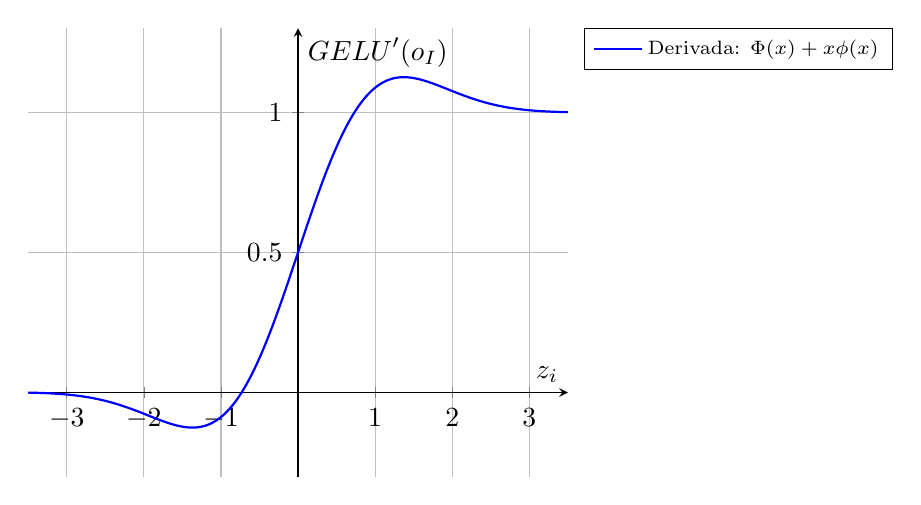
\begin{tikzpicture}
        \begin{axis}[
            xlabel={$z_i$},
            ylabel={$\text{GELU}'(o_I)$},
            xmin=-3.5, xmax=3.5,
            ymin=-0.3, ymax=1.3,
            axis lines=middle,
            grid=major,
            legend pos=outer north east,
            legend style={font=\scriptsize}
        ]
        
        % Plota a derivada usando uma aproximação para Phi(x)
        % Phi(x) ~= 1/(1+exp(-1.702*x))
        \addplot[blue, thick, domain=-3.5:3.5, samples=100, smooth] 
            {(1/(1+exp(-1.702*x))) + x * (1/sqrt(2*pi)) * exp(-x^2/2)};
        \addlegendentry{Derivada: $\Phi(x) + x\phi(x)$}
        
        \end{axis}
    \end{tikzpicture}
    \caption{Gráfico da derivada da função de ativação Gaussian Error Linear Unit (GELU).}
    \label{fig:gelu-derivada}
    \fonte{O autor (2025).}
\end{figure}

Ainda no artigo \textit{Gaussian Error Linear Units (GELUs)}, os autores discutem outras informações úteis da Gaussian Error Linear Unit para serem considerados ao construir uma rede neural com essa função de ativação, o primeiro deles é de que é recomendado o uso de um otimizador com momentum quando estiver treinando uma rede com a GELU \parencite{GELUArticle}. Em segundo lugar, \textcite{GELUArticle}, destacam que é importante utilizar uma aproximação próxima da distribuição acumulativa da distribuição gaussiana, entretanto, funções como a sigmoide, são uma aproximação acumulativa da distribuição normal, contudo, a SiLU mesmo performando pior que a GELU, ainda sim, é capaz de performar melhor que outras retificadoras como a ELU e a ReLU nos testes realizados pelos autores, assim, faz necessário o uso de novas aproximações, como as vistas nas expressões \ref{eq:gelu-aproximacoes} e \ref{eq:gelu-aproximacoes-sigmoide}.

\medskip
\begin{center}
 * * *
\end{center}
\medskip

\textbf{Algumas Aplicações da Gaussian Error Linear Unit em Redes Neurais}
\vspace{1em} 

\begin{itemize}
    \item \textbf{Aplicação 1 (Área):}
    \item \textbf{Aplicação 2 (Área):}
    \item \textbf{Aplicação 3 (Área):}
    \item \textbf{Aplicação 4 (Área):}
\end{itemize}

\medskip
\begin{center}
 * * *
\end{center}
\medskip

\subsection{Swish} \index{Funções de Ativação!Swish}

\begin{equacaodestaque}{Swish}
    \mathcal{A}_{\text{Swish}}(z_i) = z_i \cdot \sigma(z_i) = z_i \frac{1}{1 + e^{-z_i}}
    \label{eq:swish}
\end{equacaodestaque}

\begin{figure}[htbp]
    \centering
    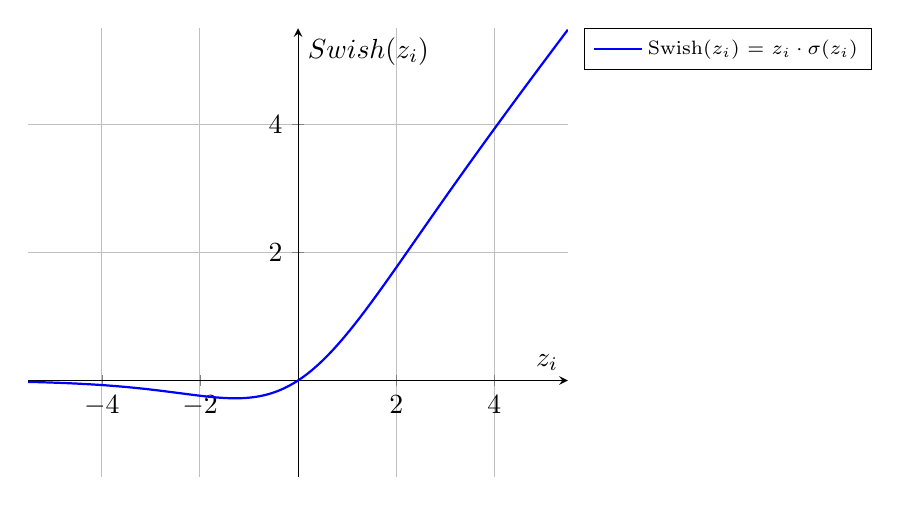
\begin{tikzpicture}
        \begin{axis}[
            xlabel={$z_i$},
            ylabel={$\text{Swish}(z_i)$},
            xmin=-5.5, xmax=5.5,
            ymin=-1.5, ymax=5.5,
            axis lines=middle,
            grid=major,
            legend pos=outer north east,
            legend style={font=\scriptsize}
        ]
        % Plota a função Swish: x * (1 / (1 + exp(-x)))
        \addplot[blue, thick, domain=-5.5:5.5, samples=100, smooth] 
            {x / (1 + exp(-x))};
        \addlegendentry{Swish($z_i$) = $z_i \cdot \sigma(z_i)$}
        
        \end{axis}
    \end{tikzpicture}
    \caption{Gráfico da função de ativação Swish.}
    \label{fig:swish}
    \fonte{O autor (2025).}
\end{figure}

\medskip
\begin{center}
 * * *
\end{center}
\medskip

\textbf{Características da Swish}
\vspace{1em}

\begin{itemize}
    \item \textbf{Característica 1:}
    \item \textbf{Característica 2:}
    \item \textbf{Característica 3:}
\end{itemize}

\medskip
\begin{center}
 * * *
\end{center}
\medskip

\begin{equacaodestaque}{Derivada Swish}
    \frac{d}{dz_i} [\mathcal{A}_{\text{Swish}}](z_i) = \text{Swish}(z_i) + \sigma(z_i)(1 - \text{Swish}(z_i))
    \label{eq:swish-derivada}
\end{equacaodestaque}

\begin{figure}[htbp]
    \centering
    \begin{tikzpicture}
        \begin{axis}[
            xlabel={$z_i$},
            ylabel={$\text{Swish}'(z_i)$},
            xmin=-5.5, xmax=5.5,
            ymin=-0.3, ymax=1.3,
            axis lines=middle,
            grid=major,
            legend pos=outer north east,
            legend style={font=\scriptsize}
        ]
        
        % Plota a derivada da função Swish
        % Swish'(x) = Swish(x) + sigmoid(x)*(1 - Swish(x))
        \addplot[orange, thick, domain=-5.5:5.5, samples=101, smooth] 
            { (x / (1 + exp(-x))) + (1 / (1 + exp(-x))) * (1 - (x / (1 + exp(-x)))) };
        \addlegendentry{$\text{Swish}'(z_i) = \text{Swish}(z_i) + \sigma(z_i)(1-\text{Swish}(z_i))$}
        
        \end{axis}
    \end{tikzpicture}
    \caption{Gráfico da derivada da função de ativação Swish.}
    \label{fig:swish-derivada}
    \fonte{O autor (2025).}
\end{figure}

\medskip
\begin{center}
 * * *
\end{center}
\medskip

\textbf{Algumas Aplicações da Swish em Redes Neurais}
\vspace{1em}

\begin{itemize}
    \item \textbf{Aplicação 1 (Área):}
    \item \textbf{Aplicação 2 (Área):}
    \item \textbf{Aplicação 3 (Área):}
    \item \textbf{Aplicação 4 (Área):}
\end{itemize}

\medskip
\begin{center}
 * * *
\end{center}
\medskip

\subsection{Hard-Swish (h-swish)} \index{Funções de Ativação!Hard-Swish (h-swish)}

\begin{equacaodestaque}{Hard-Swish}
    \mathcal{A}_{\text{h-Swish}}(z_i) = z_i \cdot \frac{\text{ReLU6}(z_i + 3)}{6}
    \label{eq:h-swish}
\end{equacaodestaque}

\begin{figure}[htbp]
    \centering
    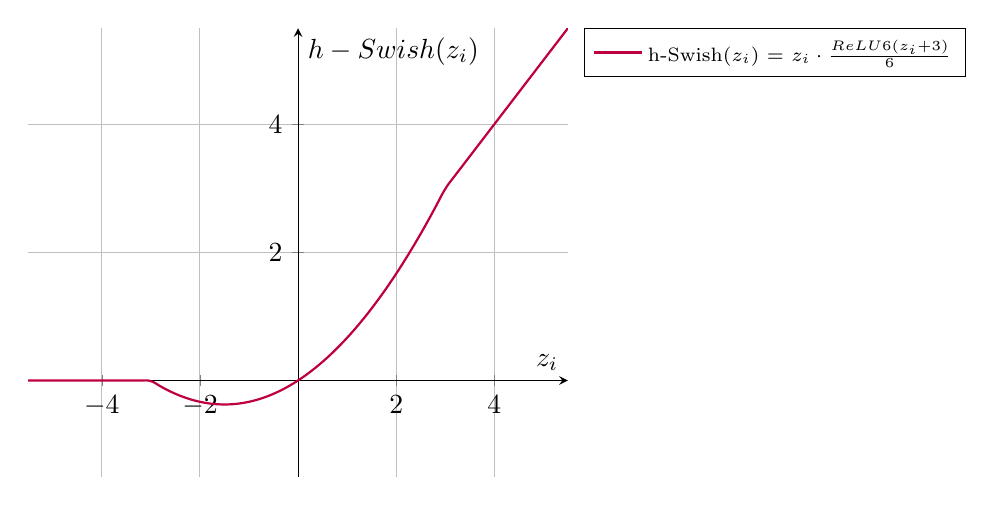
\begin{tikzpicture}
        \begin{axis}[
            xlabel={$z_i$},
            ylabel={$\text{h-Swish}(z_i)$},
            xmin=-5.5, xmax=5.5,
            ymin=-1.5, ymax=5.5,
            axis lines=middle,
            grid=major,
            legend pos=outer north east,
            legend style={font=\scriptsize}
        ]
        % Plota a função Hard-Swish: x * ReLU6(x + 3) / 6
        % ReLU6(x) = min(max(0, x), 6)
        \addplot[purple, thick, domain=-5.5:5.5, samples=100, smooth] 
            {x * min(max(0, x + 3), 6) / 6};
        \addlegendentry{h-Swish($z_i$) = $z_i \cdot \frac{\text{ReLU6}(z_i + 3)}{6}$}
        
        \end{axis}
    \end{tikzpicture}
    \caption{Gráfico da função de ativação Hard-Swish.}
    \label{fig:h-swish}
    \fonte{O autor (2025).}
\end{figure}

\medskip
\begin{center}
 * * *
\end{center}
\medskip

\textbf{Características da Hard Swish}
\vspace{1em}

\begin{itemize}
    \item \textbf{Característica 1:}
    \item \textbf{Característica 2:}
    \item \textbf{Característica 3:}
\end{itemize}

\medskip
\begin{center}
 * * *
\end{center}
\medskip

\begin{equacaodestaque}{Derivada Hard-Swish}
    \frac{d}{dz_i} [\mathcal{A}_{\text{h-Swish}}](z_i) = \begin{cases} 0 & \text{se } z_i \le -3 \\ \frac{2z_i + 3}{6} & \text{se } -3 < z_i < 3 \\ 1 & \text{se } z_i \ge 3 \end{cases}
    \label{eq:h-swish-derivada}
\end{equacaodestaque}

\begin{figure}[htbp]
    \centering
    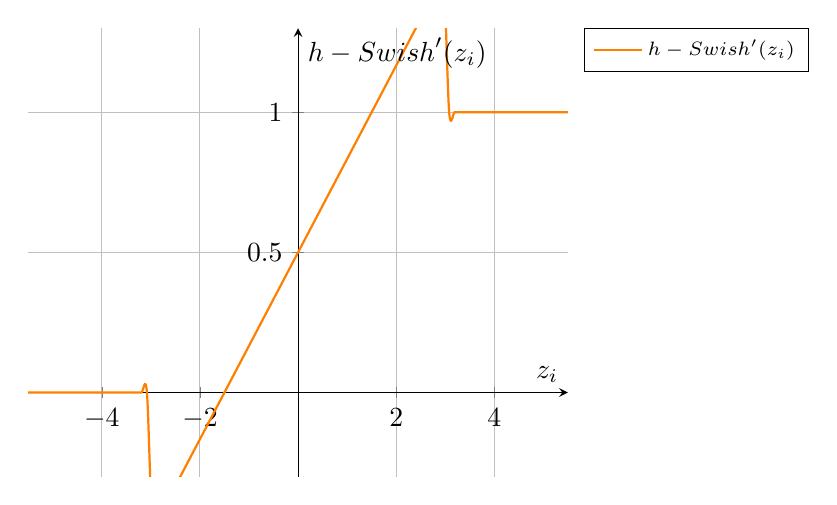
\begin{tikzpicture}
        \begin{axis}[
            xlabel={$z_i$},
            ylabel={$\text{h-Swish}'(z_i)$},
            xmin=-5.5, xmax=5.5,
            ymin=-0.3, ymax=1.3,
            axis lines=middle,
            grid=major,
            legend pos=outer north east,
            legend style={font=\scriptsize}
        ]
        
        % Plota a derivada da função Hard-Swish
        \addplot[orange, thick, domain=-5.5:5.5, samples=101, smooth] 
            { (x <= -3) ? 0 : ((x >= 3) ? 1 : ( (2*x + 3) / 6 )) };
        \addlegendentry{$\text{h-Swish}'(z_i)$}
        
        \end{axis}
    \end{tikzpicture}
    \caption{Gráfico da derivada da função de ativação Hard-Swish.}
    \label{fig:h-swish-derivada}
    \fonte{O autor (2025).}
\end{figure}

\medskip
\begin{center}
 * * *
\end{center}
\medskip

\textbf{Algumas Aplicações da Hard Swish em Redes Neurais}
\vspace{1em}

\begin{itemize}
    \item \textbf{Aplicação 1 (Área):}
    \item \textbf{Aplicação 2 (Área):}
    \item \textbf{Aplicação 3 (Área):}
    \item \textbf{Aplicação 4 (Área):}
\end{itemize}

\medskip
\begin{center}
 * * *
\end{center}
\medskip

\subsection{Mish} \index{Funções de Ativação!Mish}

\begin{equacaodestaque}{Mish}
    \mathcal{A}_{\text{Mish}}(z_i) = z_i \cdot \tanh(\text{softplus}(z_i)) = z_i \cdot \tanh(\ln(1 + e^{z_i}))
    \label{eq:mish}
\end{equacaodestaque}

\begin{figure}[htbp]
    \centering
    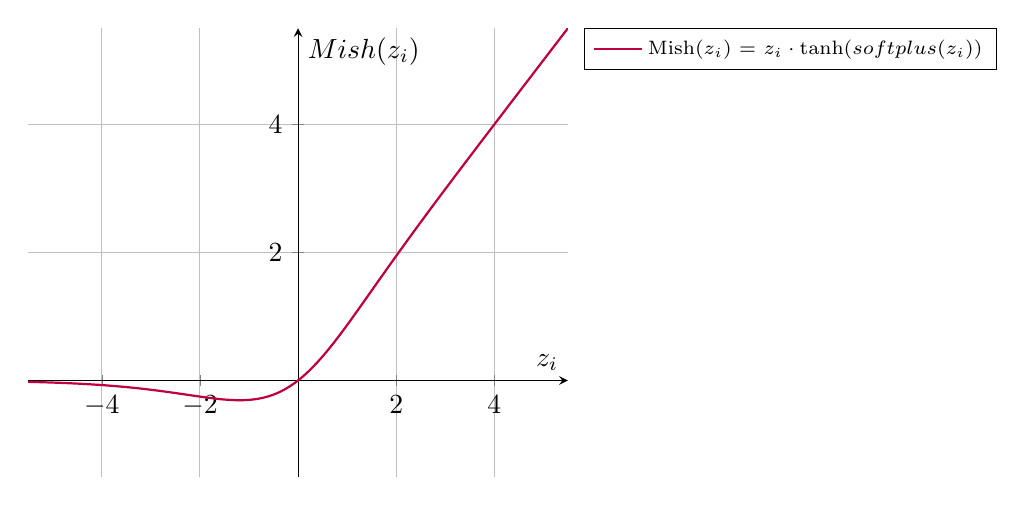
\begin{tikzpicture}
        \begin{axis}[
            xlabel={$z_i$},
            ylabel={$\text{Mish}(z_i)$},
            xmin=-5.5, xmax=5.5,
            ymin=-1.5, ymax=5.5,
            axis lines=middle,
            grid=major,
            legend pos=outer north east,
            legend style={font=\scriptsize}
        ]
        % Plota a função Mish: x * tanh(ln(1 + exp(x)))
        \addplot[purple, thick, domain=-5.5:5.5, samples=100, smooth] 
            {x * tanh(ln(1 + exp(x)))};
        \addlegendentry{Mish($z_i$) = $z_i \cdot \tanh(\text{softplus}(z_i))$}
        
        \end{axis}
    \end{tikzpicture}
    \caption{Gráfico da função de ativação Mish.}
    \label{fig:mish}
    \fonte{O autor (2025).}
\end{figure}

\medskip
\begin{center}
 * * *
\end{center}
\medskip

\textbf{Características da Mish}
\vspace{1em}

\begin{itemize}
    \item \textbf{Característica 1:}
    \item \textbf{Característica 2:}
    \item \textbf{Característica 3:}
\end{itemize}

\medskip
\begin{center}
 * * *
\end{center}
\medskip

\begin{equacaodestaque}{Derivada Mish}
    \frac{d}{dz_i} [\mathcal{A}_{\text{Mish}}](z_i) = \tanh(\omega) + z_i \sigma(z_i) \text{sech}^2(\omega) \\
    \text{onde } \omega = \text{softplus}(z_i) \text{ e } \sigma(z_i) \text{ é a função sigmoide.}
    \label{eq:mish-derivada}
\end{equacaodestaque}

\begin{figure}[htbp]
    \centering
    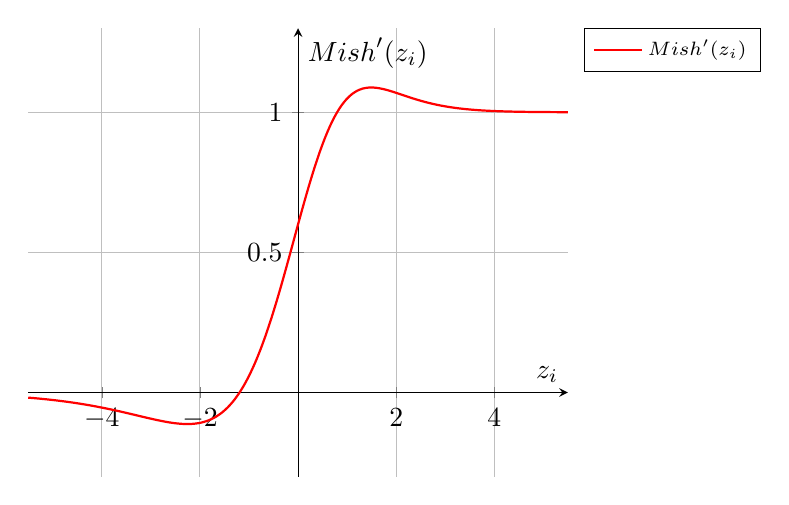
\begin{tikzpicture}
        \begin{axis}[
            xlabel={$z_i$},
            ylabel={$\text{Mish}'(z_i)$},
            xmin=-5.5, xmax=5.5,
            ymin=-0.3, ymax=1.3,
            axis lines=middle,
            grid=major,
            legend pos=outer north east,
            legend style={font=\scriptsize}
        ]
        
        % Plota a derivada da função Mish
        % Mish'(x) = tanh(sp(x)) + x * sigmoid(x) * sech^2(sp(x))
        % sp(x) = ln(1 + exp(x))
        % sigmoid(x) = 1 / (1 + exp(-x))
        % sech^2(x) = (1 / cosh(x))^2
        \addplot[red, thick, domain=-5.5:5.5, samples=101, smooth] 
            { tanh(ln(1 + exp(x))) + x * (1 / (1 + exp(-x))) * (1 / cosh(ln(1 + exp(x))))^2 };
        \addlegendentry{$\text{Mish}'(z_i)$}
        
        \end{axis}
    \end{tikzpicture}
    \caption{Gráfico da derivada da função de ativação Mish.}
    \label{fig:mish-derivada}
    \fonte{O autor (2025).}
\end{figure}

\medskip
\begin{center}
 * * *
\end{center}
\medskip

\textbf{Algumas Aplicações da Mish em Redes Neurais}
\vspace{1em}

\begin{itemize}
    \item \textbf{Aplicação 1 (Área):}
    \item \textbf{Aplicação 2 (Área):}
    \item \textbf{Aplicação 3 (Área):}
    \item \textbf{Aplicação 4 (Área):}
\end{itemize}

\medskip
\begin{center}
 * * *
\end{center}
\medskip

\subsection{Hard-Mish (h-mish)} \index{Funções de Ativação!Hard-Mish (h-mish)}

\begin{equacaodestaque}{Hard-Mish}
    \mathcal{A}_{\text{h-Mish}}(z_i) = \frac{z_i}{2} \cdot \min(\max(z_i + 2, 0), 2)
    \label{eq:h-mish}
\end{equacaodestaque}

\begin{figure}[htbp]
    \centering
    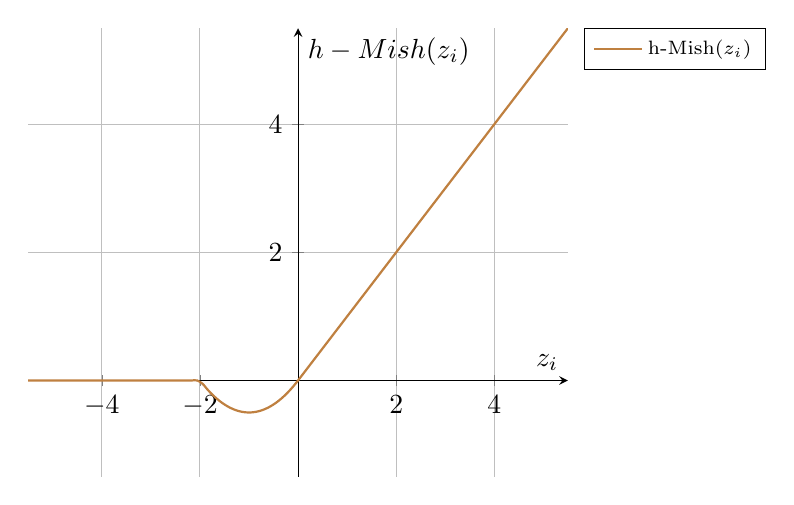
\begin{tikzpicture}
        \begin{axis}[
            xlabel={$z_i$},
            ylabel={$\text{h-Mish}(z_i)$},
            xmin=-5.5, xmax=5.5,
            ymin=-1.5, ymax=5.5,
            axis lines=middle,
            grid=major,
            legend pos=outer north east,
            legend style={font=\scriptsize}
        ]
        % Plota a função Hard-Mish: x/2 * min(max(x + 2, 0), 2)
        \addplot[brown, thick, domain=-5.5:5.5, samples=100, smooth] 
            {x * min(max(0, x + 2), 2) / 2};
        \addlegendentry{h-Mish($z_i$)}
        
        \end{axis}
    \end{tikzpicture}
    \caption{Gráfico da função de ativação Hard-Mish.}
    \label{fig:h-mish}
    \fonte{O autor (2025).}
\end{figure}

\medskip
\begin{center}
 * * *
\end{center}
\medskip

\textbf{Características da Hard Mish}
\vspace{1em}

\begin{itemize}
    \item \textbf{Característica 1:}
    \item \textbf{Característica 2:}
    \item \textbf{Característica 3:}
\end{itemize}

\medskip
\begin{center}
 * * *
\end{center}
\medskip

\begin{equacaodestaque}{Derivada Hard-Mish}
    \frac{d}{dz_i} [\mathcal{A}_{\text{h-Mish}}](z_i) = \begin{cases} 0 & \text{se } z_i \le -2 \\ z_i + 1 & \text{se } -2 < z_i < 0 \\ 1 & \text{se } z_i \ge 0 \end{cases}
    \label{eq:h-mish-derivada}
\end{equacaodestaque}

\begin{figure}[htbp]
    \centering
    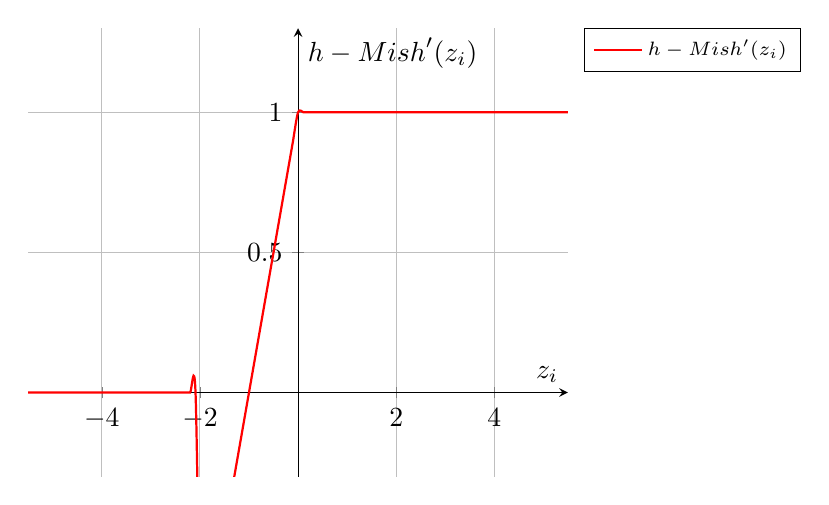
\begin{tikzpicture}
        \begin{axis}[
            xlabel={$z_i$},
            ylabel={$\text{h-Mish}'(z_i)$},
            xmin=-5.5, xmax=5.5,
            ymin=-0.3, ymax=1.3,
            axis lines=middle,
            grid=major,
            legend pos=outer north east,
            legend style={font=\scriptsize}
        ]
        
        % Plota a derivada da função Hard-Mish
        \addplot[red, thick, domain=-5.5:5.5, samples=101, smooth] 
            { (x <= -2) ? 0 : ((x >= 0) ? 1 : (x + 1)) };
        \addlegendentry{$\text{h-Mish}'(z_i)$}
        
        \end{axis}
    \end{tikzpicture}
    \caption{Gráfico da derivada da função de ativação Hard-Mish.}
    \label{fig:h-mish-derivada}
    \fonte{O autor (2025).}
\end{figure}

\medskip
\begin{center}
 * * *
\end{center}
\medskip

\textbf{Algumas Aplicações da Hard Mish em Redes Neurais}
\vspace{1em}

\begin{itemize}
    \item \textbf{Aplicação 1 (Área):}
    \item \textbf{Aplicação 2 (Área):}
    \item \textbf{Aplicação 3 (Área):}
    \item \textbf{Aplicação 4 (Área):}
\end{itemize}

\medskip
\begin{center}
 * * *
\end{center}
\medskip

\section{Funções Para Camadas de Saída}

\subsection{Softmax}

\begin{equacaodestaque}{Softmax}
    \mathcal{A}_{\text{Softmax}}(z_i) = \frac{e^{z_i}}{\sum_{j=1}^{K} e^{z_j}}
    \label{eq:softmax}
\end{equacaodestaque}

\begin{equacaodestaque}{Derivada Softmax}
    \frac{\partial [\mathcal{A}_{\text{Softmax}}](z_i)}{\partial z_j} = 
    \begin{cases} 
      \text{Softmax}(z_i)(1 - \text{Softmax}(z_i)) & \text{se } i = j \\
      - \text{Softmax}(z_i)\text{Softmax}(z_j) & \text{se } i \neq j
    \end{cases}
    \label{eq:softmax-derivada}
\end{equacaodestaque}

\subsection{Identidade (Linear)}

\begin{equacaodestaque}{Identidade}
    \mathcal{A}_{\text{Linear}}(z_i) = z_i
    \label{eq:linear}
\end{equacaodestaque}

\begin{figure}[htbp]
    \centering
    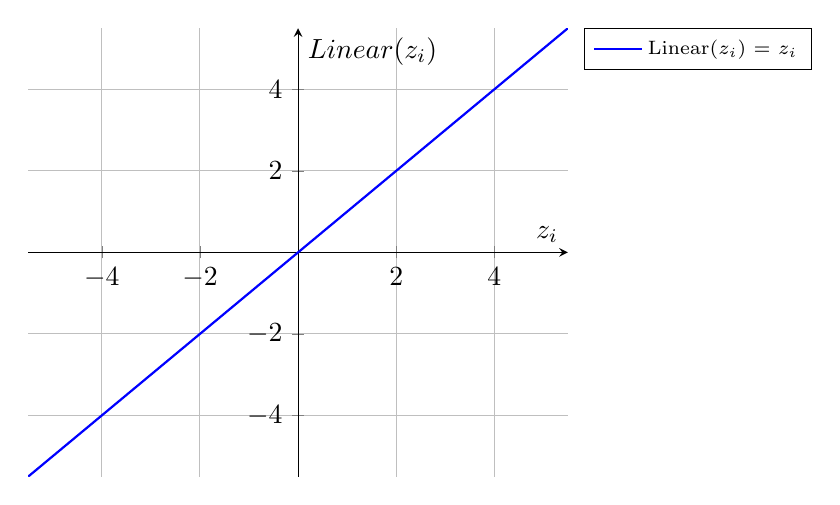
\begin{tikzpicture}
        \begin{axis}[
            xlabel={$z_i$},
            ylabel={$\text{Linear}(z_i)$},
            xmin=-5.5, xmax=5.5,
            ymin=-5.5, ymax=5.5, % Ajustado para y=x
            axis lines=middle,
            grid=major,
            legend pos=outer north east,
            legend style={font=\scriptsize}
        ]
        % Plota a função Identidade: y = x
        \addplot[blue, thick, domain=-5.5:5.5, samples=10, smooth] 
            {x};
        \addlegendentry{Linear($z_i$) = $z_i$}
        
        \end{axis}
    \end{tikzpicture}
    \caption{Gráfico da função de ativação Linear (Identidade).}
    \label{fig:linear}
    \fonte{O autor (2025).}
\end{figure}

\begin{equacaodestaque}{Derivada Identidade}
    \frac{d}{dz_i} [\mathcal{A}_{\text{Linear}}](z_i) = 1
    \label{eq:linear-derivada}
\end{equacaodestaque}

\begin{figure}[htbp]
    \centering
    \begin{tikzpicture}
        \begin{axis}[
            xlabel={$z_i$},
            ylabel={$\text{Linear}'(z_i)$},
            xmin=-5.5, xmax=5.5,
            ymin=-0.3, ymax=1.3,
            ytick={1}, % Útil para mostrar que é constante
            axis lines=middle,
            grid=major,
            legend pos=outer north east,
            legend style={font=\scriptsize}
        ]
        
        % Plota a derivada da função Linear: y = 1
        \addplot[orange, thick, domain=-5.5:5.5, samples=10, smooth] 
            {1};
        \addlegendentry{$\text{Linear}'(z_i) = 1$}
        
        \end{axis}
    \end{tikzpicture}
    \caption{Gráfico da derivada da função de ativação Linear.}
    \label{fig:linear-derivada}
    \fonte{O autor (2025).}
\end{figure}

\subsection{Softplus}

\begin{equacaodestaque}{Softplus}
    \mathcal{A}_{\text{Softplus}}(z_i) = \ln(1 + e^{z_i})
    \label{eq:softplus}
\end{equacaodestaque}

\begin{figure}[htbp]
    \centering
    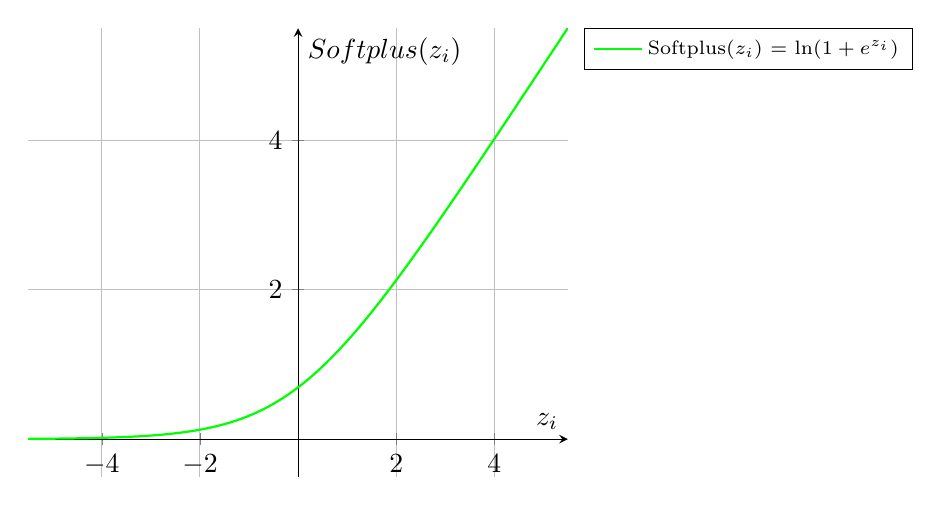
\begin{tikzpicture}
        \begin{axis}[
            xlabel={$z_i$},
            ylabel={$\text{Softplus}(z_i)$},
            xmin=-5.5, xmax=5.5,
            ymin=-0.5, ymax=5.5, % Eixo do template funciona bem
            axis lines=middle,
            grid=major,
            legend pos=outer north east,
            legend style={font=\scriptsize}
        ]
        % Plota a função Softplus: ln(1 + exp(x))
        \addplot[green, thick, domain=-5.5:5.5, samples=100, smooth] 
            {ln(1 + exp(x))};
        \addlegendentry{Softplus($z_i$) = $\ln(1 + e^{z_i})$}
        
        \end{axis}
    \end{tikzpicture}
    \caption{Gráfico da função de ativação Softplus.}
    \label{fig:softplus}
    \fonte{O autor (2025).}
\end{figure}

\begin{equacaodestaque}{Derivada Softplus}
    \frac{d}{dz_i} [\mathcal{A}_{\text{Softplus}}](z_i) = \frac{e^{z_i}}{1 + e^{z_i}} = \frac{1}{1 + e^{-z_i}} = \sigma(z_i)
    \label{eq:softplus-derivada}
\end{equacaodestaque}

\begin{figure}[htbp]
    \centering
    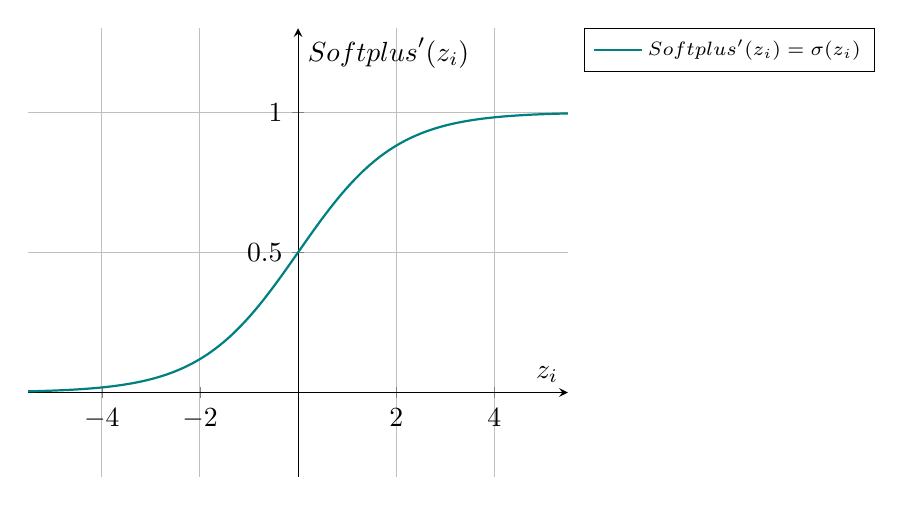
\begin{tikzpicture}
        \begin{axis}[
            xlabel={$z_i$},
            ylabel={$\text{Softplus}'(z_i)$},
            xmin=-5.5, xmax=5.5,
            ymin=-0.3, ymax=1.3,
            axis lines=middle,
            grid=major,
            legend pos=outer north east,
            legend style={font=\scriptsize}
        ]
        
        % Plota a derivada da função Softplus (função Sigmoide)
        \addplot[teal, thick, domain=-5.5:5.5, samples=101, smooth] 
            { 1 / (1 + exp(-x)) };
        \addlegendentry{$\text{Softplus}'(z_i) = \sigma(z_i)$}
        
        \end{axis}
    \end{tikzpicture}
    \caption{Gráfico da derivada da função de ativação Softplus, que é a função Sigmoide.}
    \label{fig:softplus-derivada}
    \fonte{O autor (2025).}
\end{figure}

\subsection{Exponencial (exp)}

\begin{equacaodestaque}{Exponencial}
    \mathcal{A}_{\text{Exp}}(z_i) = e^{z_i}
    \label{eq:exp}
\end{equacaodestaque}

\begin{figure}[htbp]
    \centering
    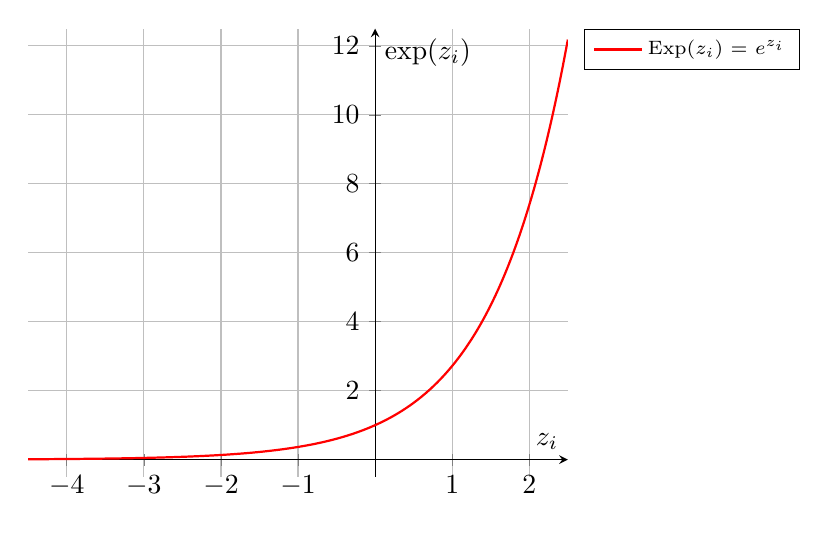
\begin{tikzpicture}
        \begin{axis}[
            xlabel={$z_i$},
            ylabel={$\exp(z_i)$},
            xmin=-4.5, xmax=2.5, % Eixos ajustados
            ymin=-0.5, ymax=12.5, % Eixos ajustados
            axis lines=middle,
            grid=major,
            legend pos=outer north east,
            legend style={font=\scriptsize}
        ]
        % Plota a função Exponencial: exp(x)
        \addplot[red, thick, domain=-4.5:2.5, samples=100, smooth] 
            {exp(x)};
        \addlegendentry{Exp($z_i$) = $e^{z_i}$}
        
        \end{axis}
    \end{tikzpicture}
    \caption{Gráfico da função de ativação Exponencial (eixos ajustados).}
    \label{fig:exp}
    \fonte{O autor (2025).}
\end{figure}

\begin{equacaodestaque}{Derivada Exponencial}
    \frac{d}{dz_i} [\mathcal{A}_{\text{Exp}}](z_i) = e^{z_i}
    \label{eq:exp-derivada}
\end{equacaodestaque}

\begin{figure}[htbp]
    \centering
    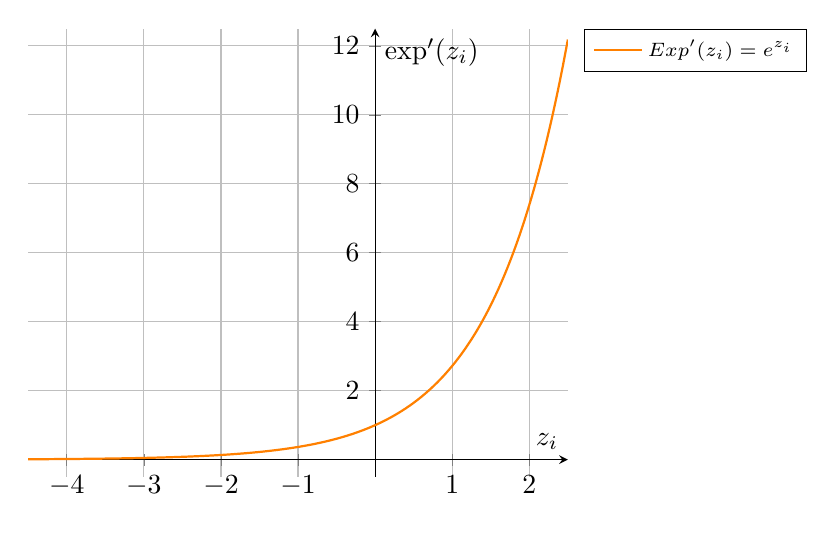
\begin{tikzpicture}
        \begin{axis}[
            xlabel={$z_i$},
            ylabel={$\exp'(z_i)$},
            xmin=-4.5, xmax=2.5, % Eixos ajustados
            ymin=-0.5, ymax=12.5, % Eixos ajustados
            axis lines=middle,
            grid=major,
            legend pos=outer north east,
            legend style={font=\scriptsize}
        ]
        
        % Plota a derivada da função Exponencial: exp(x)
        \addplot[orange, thick, domain=-4.5:2.5, samples=101, smooth] 
            {exp(x)};
        \addlegendentry{$\text{Exp}'(z_i) = e^{z_i}$}
        
        \end{axis}
    \end{tikzpicture}
    \caption{Gráfico da derivada da função de ativação Exponencial (eixos ajustados).}
    \label{fig:exp-derivada}
    \fonte{O autor (2025).}
\end{figure}



